\documentclass{article}
\usepackage[utf8]{inputenc}


\title{Curso Openscad}
\author{Pablo Vivar Colina}
\date{Agosto 2017}

%IDIOMA
\usepackage[spanish.mexico]{babel}

\usepackage{natbib}
\usepackage{graphicx}

%ELEGANTE
\usepackage{fancyhdr}
\pagestyle{fancy}

%\usepackage[top=2cm,bottom=2cm,left=1cm,right=1cm]{geometry}
\begin{titlepage}
     \begin{center}
     
     %#######INCLUIR LOGO#########
	
	
	\Large Universidad Nacional Autónoma de México\\[1.5cm]
        	
        	%#######INCLUIR LOGO#########
        	%\includegraphics[width=0.1\textwidth]{FI}\\[1cm]
        
        \Large Facultad de Ingeniería\\[1.5cm]
        %\Large División de Ciencias Básicas\\[1cm]
         \Large Laboratorio de Investigación y Desarrollo de Software Libre\\[1.5cm]
         
        \Large
        Cusrso de Introducción de modelado parametrizable con OpenSCAD\\[1.5cm]
        \Large Semestre 2018-1\\[1.5cm]
        
        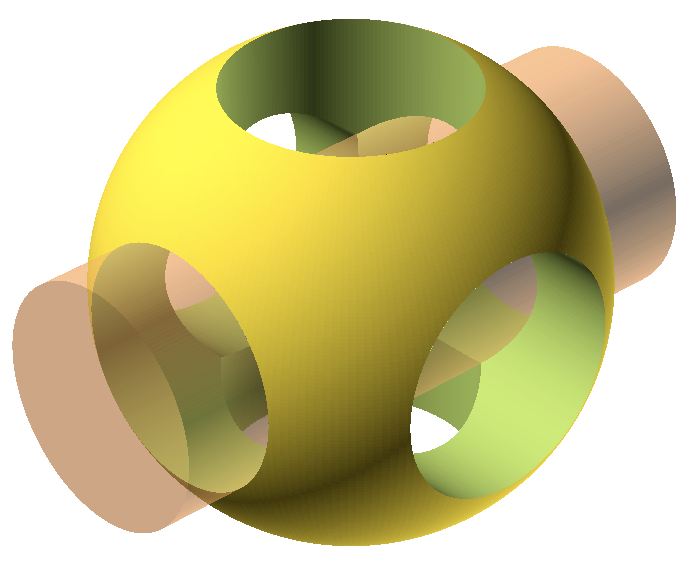
\includegraphics[width=0.5\textwidth]{OpenSCAD-logo.png}
        
        \Large Programa\\[1cm]
         \Large Pablo Vivar Colina\\[1cm]
        %\Large Movimiento Ondulatorio\\[1cm]

         %Texto a la derecha
 %         \begin{flushright}
%\footnotesize  Grupo 01\\[0.5cm]
%\footnotesize Brigada: 1\\[0.5cm]
%\footnotesize Integrantes:\\[0.5cm]
%Alumno\\[0.5cm]
%\footnotesize Montoya Rangel Luis Rodrigo\\[0.5cm]
%\footnotesize Vivar Colina Pablo\\[0.5cm]
% \end{flushright}
    %Texto a la izquierda
          \begin{flushleft}
        \footnotesize Ciudad Universitaria Septiembre de 2017.\\
          \end{flushleft}
         
          
        %\vfill
        %\today
   \end{center}
\end{titlepage}

\begin{document}

%\maketitle



\tableofcontents

%\listoffigures %*PATENTE
%\listoftables
.\\[3cm]

\section{Introducción}

En el desarrollo de prototipos en ingeniería es importante el desarrollo de modelos 3D para poder visualizar las piezas que se desean manufacturar que si existen errores, éstos puedan ser corregidos. En éste proceso se necesita tiempo y la habilidad de la persona que está desarrollando éstos modelos para lograr corregir éstos errores de manera eficiente.\\

OpenSCAD es una plataforma de desarrollo de dibujos 2D y 3D en donde los modelos son programados a través de líneas de código,y éstos pueden ser parametrizables.\\

OpenSCAD es una aplicación libre para crear objetos sólidos de CAD. No es un editor interactivo sino un compilador 3D basado en un lenguaje de descripción textual. Un documento de OpenSCAD especifica primitivas geométricas y define como son modificadas y manipuladas para reproducir un modelo 3D. OpenSCAD está disponible para Windows, Linux y OS X. OpenSCAD realiza geometría constructiva de sólidos (CSG).\citep{WikiOpensCAD}


\section{Programa}

\subsection{Conceptos}

    \begin{enumerate}
    
    \item Objetos

Los objetos son las piezas de construcción para realizar modelos, creadas en primitivas 2D y 3D, los objetos deben finalizar con punto y coma ';'.\citep{WikiOpensCADLanguage}

    \item Acciones
    
    Las instancias de acción incluye la creación de objetos a partir de primitivas y asignando valores a las variables. Las instancias de acción también finalizan con punto y coma.\citep{WikiOpensCADLanguage}
    
    \item Operadores
    
    Operadores, o transformaciones, modifica la localización, color u otras propiedades de los objetos. Los operadores usan llaves '{}' cuando su campo de acción cubre más de una acción. Más de un operador puede ser usado para la misma acción o grupo de acciones. Operadores múltiples son procesados de Derecha a Izquierda, eso quiere decir que el operador más cercano a la acción es procesado primero. Los operadores no terminan con punto  coma ';', pero las acciones individuales pueden contenerla.\citep{WikiOpensCADLanguage}
    
    \end{enumerate}
    
 

\subsection{Sintaxis}

\subsubsection{Variables}

Objetivo: Expliacición de las variables en el entorno parametrizable.\citep{OpenSCS}\\

Las variables de OpenSCAD son creadas en instancia con un nombre o identificador, asignando una expresión y un punto y coma. El rol de los arreglos, encontrado en muchos lenguajes imperativos, es manejado en OpenSCAD via vectores.\citep{WikiOpensCADLanguage}\\

\begin{figure}[h!]
\begin{verbatim}

var = 25;
xx = 1.25 * cos(50);
y = 2*xx+var;
logic = true;
MyString = "This is a string";
a_vector = [1,2,3];
rr = a_vector[2];      // member of vector
range1 = [-1.5:0.5:3]; // for() loop range
xx = [0:5];            // alternate for() loop range

\end{verbatim}
\caption{Diferentes formas de representar variables en OpenSCAD}
\end{figure}


\subsection{2D}

\subsubsection{Círculos}

Objetivo: Empleo y declaración de círculos.\citep{OpenSCS}\\

Para crear círculos todos los parámetros excepto la r deben ser nombrados, los círculos se crean en el origen.\citep{WikiOpensCADLanguage}\\

\begin{verbatim}
    circle(r=radius | d=diameter);
\end{verbatim}

Parámetros:\\

r: es el radio del círculo.

La resolución del círculo está basada en el tamaño usando  \$fa o \$fs.\\

Para un círculo pequeño de alta resolución, se puede hacer un círculo grande, y reducirlo, o puedes usar el parámetro \$fn u otras variables especiales.\citep{WikiOpensCADLanguage}\\

Nota: Éstos ejemplos exceden la resolución de una impresora 3D.\citep{WikiOpensCADLanguage}\\


\begin{enumerate}
\item d: diámetro del círculo (solo en versiones después de 2014.03).
\item \$fa: ángulo mínimo (en grados) de cada fragmento.
\item \$fs: largo circunferencial mínimo de cada fragmento.
\item \$fn: fragmentos acomodados en 360 grados valores desde 3 a mayores.
\item \$fa, \$fs y \$fn deben ser nombrados.
\end{enumerate}

\begin{figure}[h!]
    \centering
   \begin{verbatim}
defaults:  circle(); 
yields:  circle(\$fn = 0, \$fa = 12, \$fs = 2, r = 1);
\end{verbatim}
    \caption{Código base del círculo}
    \label{fig:codCirculo}
\end{figure}

Como se puede apreciar en la figura \ref{fig:codCirculo} y se ha mencionado en el concepto de objeto, se puede apreciar que para generar un círculo solo hace falta una línea de código, y dentro de sus argumentos pueden ir definidos o no varios campos que le harán modificar sus características.\\

\begin{figure}[h!]
    \centering
    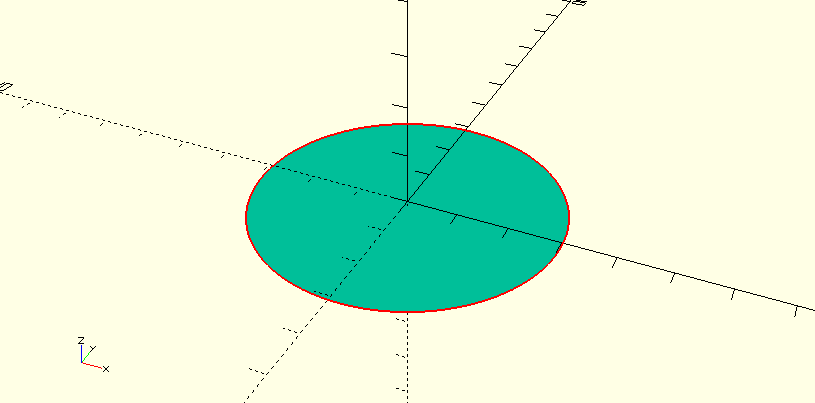
\includegraphics[width=0.5\textwidth]{Imagenes/Circulo.png}
    \caption{Ejemplo gráfico círculo}
    \label{fig:grafCirculo}
\end{figure}

En la figura \ref{fig:grafCirculo} es una representación genérica de un círculo con un radio y definición determinadas, es importante observar que el círculo se genera en el origen del sistema de coordenadas sobre el plano XY y además que es un círculo 2D.\\

\subsubsection{Cuadrado}

Objetivo: Empleo y declaración de paralelogramos.\\

Éste ejemplo sirve para crear un cuadrado o un rectángulo en el primer cuadrante. Los nombres de los argumentos son opcionales.

\begin{verbatim}
    square(size = [x, y], center = true/false);
    square(size =  x    , center = true/false);
\end{verbatim}

\begin{figure}[h!]
    \centering
    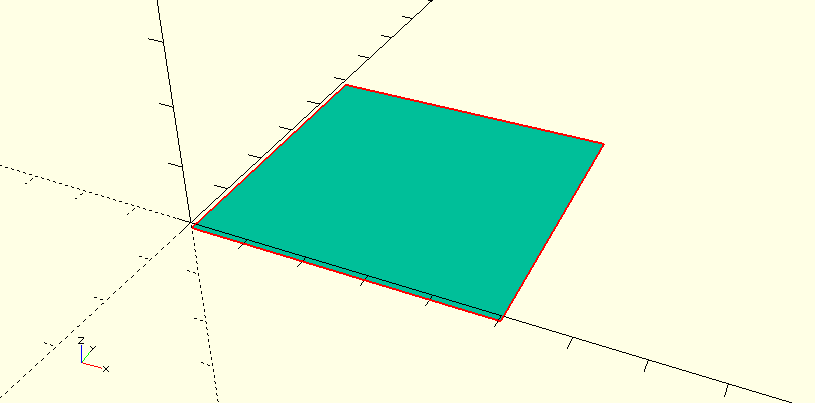
\includegraphics[width=0.5\textwidth]{Imagenes/Cuadrado.png}
    \caption{Ejemplo gráfico Cuadrado}
    \label{fig:grafCuadrado}
\end{figure}


Cuándo el centro es verdadero el cuadrado es centrado en el origen. 

\begin{figure}[h!]
    \centering
    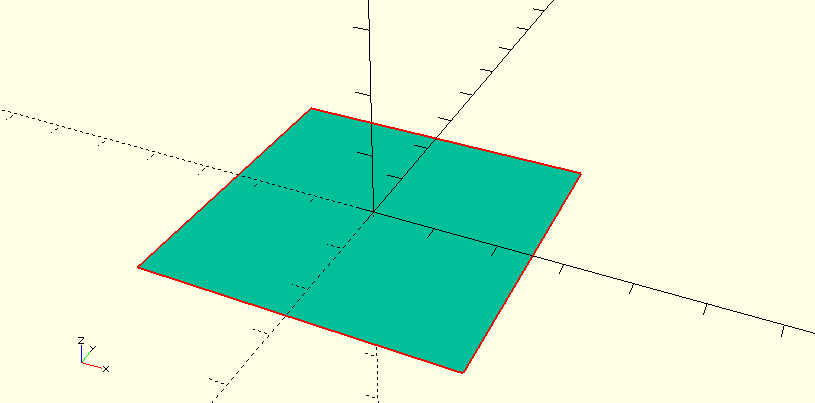
\includegraphics[width=0.5\textwidth]{Imagenes/CuadradoCentro.png}
    \caption{Ejemplo gráfico Cuadrado centrado}
    \label{fig:grafCuadradoCentro}
\end{figure}



\subsubsection{Polígonos Regulares}

Objetivo: Dibujo de polígonos regulares.\citep{OpenSCS}\\

Un polígono regular de 3 o más lados puede ser creado usando círculos (circle()) con \$fn definiendo el número de lados. El polígono es inscrito dentro del círculo con todos sus lados (y ángulos) igualmente. Una esquina apunta a la dirección "x" positiva.\citep{WikiOpensCAD}

\begin{figure}[h!]
    \centering
    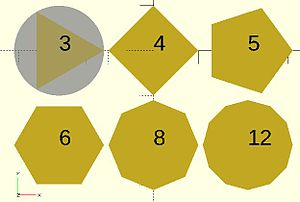
\includegraphics[width=0.5\textwidth]{Imagenes/polygon.jpg}
    \caption{Polígonos regulares}
    \label{fig:grafPolygon}
\end{figure}

\subsubsection{Polígono}

Objetivo: Dibujo de polígonos.\citep{OpenSCS}\\

Para hacer polígonos o una forma de formas múltiples, se genera a partir de coordenadas x,y. Un polígono es el objeto más poderoso 2D.
Se puede crear cualquier cosa más que los círculos y los cuadrados pueden y mucho más. Ésto incluye formas irregulares con esquinas cóncavas y convexas. Además se puede colocar agujeros dentro de la figura.\citep{WikiOpensCAD}
\\

\begin{verbatim}
    polygon(points = [ [x, y], ... ],
    paths = [ [p1, p2, p3..], ...], convexity = N);
\end{verbatim}

Parámetros:\\

\begin{enumerate}
    \item puntos:la lista de puntos x,y del polígono: Un vector de 2 vectores elementales.
    \item trayectorias por defecto: Si no hay una trayectoria en específico, todos los puntos se usarán con el orden de la lista.
    \item trayectorias por vector sencillo: para se siga una trayectoria a través de los puntos. Se usan índices desde 0 hasta n-1. Pueden ser usados en un orden diferente, usar todos o una parte de los puntos listados. 
    \item trayectorias por múltiples vectores: Crea formas primarias y secundarias. Las formas secundarias son sustraídas de las formas primarias (como diferencia). Las formas secundarias pueden ser totalmente o parcialmentecompuestas the la forma primaria.

    
\end{enumerate}

Una trayectroia cerrada es creada regresando desde el último punto especificado hacia el primero.\citep{WikiOpensCAD}
\\

\subsubsection{Texto}

Objetivo: Diferentes usos de texto.\citep{OpenSCS}\\

El módulo de texto crea textos como un dibujo 2D genérico, usando las fuentes instaladas en el sistema local o provistos como una fuente de un archivo por separado.\citep{OpenSCADtext}
\\

\begin{figure}[h!]
    \centering
    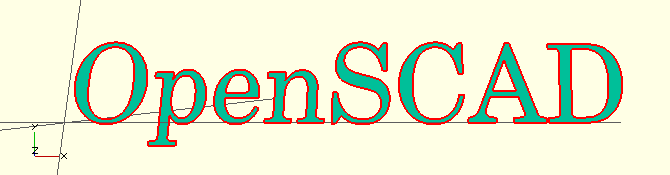
\includegraphics[scale=0.5]{Imagenes/OpenSCADtext.png}
    \caption{Ejemplo de texto en 2D}
    \label{fig:ejemploTexto}
\end{figure}


\subsection{3D}


\subsubsection{Esfera}

Objetivo: Declaración y uso de esferas.\citep{OpenSCS}\\

Crea una esfera en un origen de coordenadas de un sistema. El nombre del argumento $r$ es opcional. Para usar $d$ en vez de $r$, $d$ debe ser nombrada.\citep{OpenSCADtext}\\

Parámetros:\\

\begin{enumerate}
    \item r: Radio es el radio de la esfera. La resolucipon de la esfera debe ser basada en el tamaño de la esfera y las variables $\$fa $, $\$fs$ y $\$fn$. Para más información en éstas variables especiales consultar: OpenSCAD\_User \_Manual/Other\_Language\_Features
    \item d Diáetro es el díametro de la esfera. (Nota: d está disponible en las versiones después de la 2014.03. Debaian se encuentra detrás de ésto)
    \item $\$fa $ Fragmento de ángulo en grados
    \item $\$fs$ Fragmento de tamaño en mm
    \item $\$fn$ Resolución
\end{enumerate}

\begin{verbatim}
    default values:  sphere();  
    yields:   sphere(\$fn = 0, \$fa = 12, \$fs = 2, r = 1);
\end{verbatim}

\begin{verbatim}
    // Esto creara una esfera de alta resolucion con 2mm de radio
sphere(2,  \$fn=100); 
\end{verbatim}

\begin{verbatim}
    // tambien creara una esfera de 2mm con alta resolución,
    //esta en cambio evitara crear pequeños triangulos como pueda en los polos de la esfera
sphere(2, $fa=5, $fs=0.1);
\end{verbatim}


\begin{figure}[h!]
    \centering
    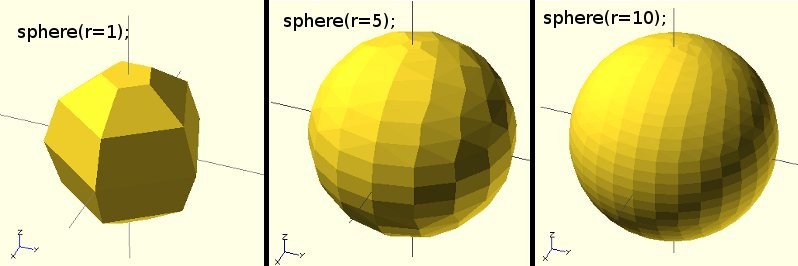
\includegraphics[scale=0.8]{Imagenes/Openscad-sphere.jpg}
    \caption{Ejemplo de resolución esferas}
    \label{fig:resEsferas}
\end{figure}


\subsubsection{Cubo}

Objetivo: Declaración y uso de paralepípedos.\citep{OpenSCS}\\

Crea un cubo en el primer octante. Cuando el centro tiene valor verdadero "true", el cubo es centrado en el origen. Los nombres de los argumentos son opcionales si se dan en el orden mostrado.\citep{WikiOpensCAD}\\

\begin{verbatim}
    cube(size = [x,y,z], center = true/false);
   cube(size =  x ,     center = true/false);
\end{verbatim}

Parámetros:\\

\begin{enumerate}
    \item tamaño: Valor sencillo, cubo con todos sus lados, arreglo de 3 valores $[x,y,x]$, cubo con dimensiones $x$,$y$ y $z4$.
    
   \item centro: el valor por defecto en falso ("false"), esto es que el cubo se desarrolla en el primer octante, con esquina en $(0,0,0)$, cuando es verdadero ("true"), el centro del cubo es centrado en el origen en: $(0,0,0)$.

\end{enumerate}

\begin{verbatim}
    default values:  cube();  
    yields:  cube(size = [1, 1, 1], center = false);
\end{verbatim}

Ejemplos:\\

\begin{figure}[h!]
    \centering
    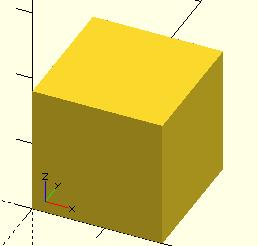
\includegraphics[scale=0.5]{Imagenes/OpenSCAD_example_Cube.jpg}
    \caption{Ejemplo de cubo generado en el primer octante}
    \label{fig:cubo_defecto}
\end{figure}

Códigos equivalentes para el ejemplo de la figura \ref{fig:cubo_defecto}:\\

\begin{verbatim}
 cube(size = 18);
 cube(18);
 cube([18,18,18]);
 .
 cube(18,false);
 cube([18,18,18],false);
 cube([18,18,18],center=false);
 cube(size = [18,18,18], center = false);
 cube(center = false,size = [18,18,18] );
\end{verbatim}

\begin{figure}[h!]
    \centering
    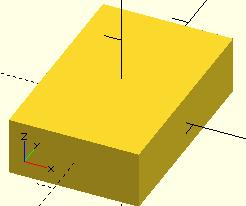
\includegraphics[scale=0.5]{Imagenes/OpenSCAD_example_Box.jpg}
    \caption{Ejemplo de cubo centrado en el origen}
    \label{fig:cubo_origen}
\end{figure}

Código equivalente para el ejemplo de la figura \ref{fig:cubo_origen}:\\

\begin{verbatim}
 cube([18,28,8],true);
 box=[18,28,8];cube(box,true);
\end{verbatim}

\subsubsection{Cilindro}

Objetivo: Declaración y uso de cilindros.\citep{OpenSCS}\\


Crea un cilindro o cono centrado alrededor del eje z. Cuando el centro es verdadero ("true"), es también centrada verticalmente a través del eje z.\citep{WikiOpensCAD}\\

Los nombres de los parámetros son opcionales si se da el orden mostrado a continuación. Si un parámetro es nombrado, todos los siguientes parámetros también deberán ser nombrados.\citep{WikiOpensCAD}\\

NOTA: Si r, d, d1, o d2 son usados, deben ser nombrados.\citep{WikiOpensCAD}\\

\begin{verbatim}
    cylinder(h = height, r1 = BottomRadius, r2 = TopRadius, center = true/false);
\end{verbatim}

Parámetros:\\

\begin{enumerate}
    \item h: altura del cilindro o cono.
    \item r: radio del cilindro. r1 = r2 =r.
    \item r1: radio, parte baja del cono.
    \item r2: radio, parte alta del cono.
    \item d: diámetro del cilindro. r1 = r2 =d/2.
    \item d1: diámetro, parte baja del cono. r1 = d1/2.
    \item d2: diámetro, parte alta del cono. r2 = d2/2.\\
    (NOTA: d,d1,d2, requiere 2014.03 o superior. Es sabido que Debian se encuentra debajo de ésto)
    \item centro:\\
    falso ("false") por defecto, z se encuetra en el rango desde 0 hasta h\\
    verdadero ("true"), z se encuentra en el rango desde -h/2 hasta +h/2
    \item \$fa: ángulo mínimo (grados) de cada fragmento.
    \item \$fs: radio circunferencial m+inimo de cada fragmento.
    \item \$fn: número fijo de fragmentos en 360 grados. Valores desde 3 o más, o sobrecarga de \$fa y \$fs\\
    
    \$fa,\$fs y \$fn deben ser nombradas
\end{enumerate}
    
    \begin{verbatim}
        defaults: cylinder();  
        yields: cylinder(\$fn = 0, \$fa = 12, \$fs = 2, h = 1, r1 = 1, r2 = 1, center = false);
    \end{verbatim}

%#######CILINDRO INCOMPLETO!!!13sept2017#######
    
\subsubsection{Polihedros}

Objetivo: Declaración y uso de Polihedros.\citep{OpenSCS}\\

\subsection{Transformaciones}

\subsubsection{Translado}

Objetivo: Uso de transformación translado.\citep{OpenSCS}\\

\subsubsection{Rotación}

Objetivo: Uso de transformación rotación. \citep{OpenSCS}\\

\subsubsection{Escala}

Objetivo: Uso de la transformación escala.\citep{OpenSCS}\\

\begin{verbatim}
   scale([1.5,0.5])circle(d=20);
\end{verbatim}

\subsubsection{Redimensionar}

Objetivo: Uso de la transformación de redimensión.\citep{OpenSCS}\\

\begin{verbatim}
     resize([30,10])circle(d=20);
\end{verbatim}

\subsubsection{Espejo}

Objetivo: Uso de la transformación espejo.\citep{OpenSCS}\\

\subsubsection{Color}

Objetivo: Uso de la transformación color.\citep{OpenSCS}\\

\subsubsection{Offset}

Objetivo: Uso de la transformación offset.\citep{OpenSCS}\\


\citep{OpenSCS}

\subsection{Operaciones Booleanas}

\subsubsection{Union}

Objetivo: Uso de la operación de Unión.\citep{OpenSCS}\\


Crea una Unión de sus nodos hijos. Ésto es la suma de todos los hijos.\citep{WikiOpensCAD}\\

Puede ser usado con objetos tanto 2D y 3D, pero no puede mezclarlos.\citep{WikiOpensCAD}\\

\begin{figure}[h!]
    \centering
    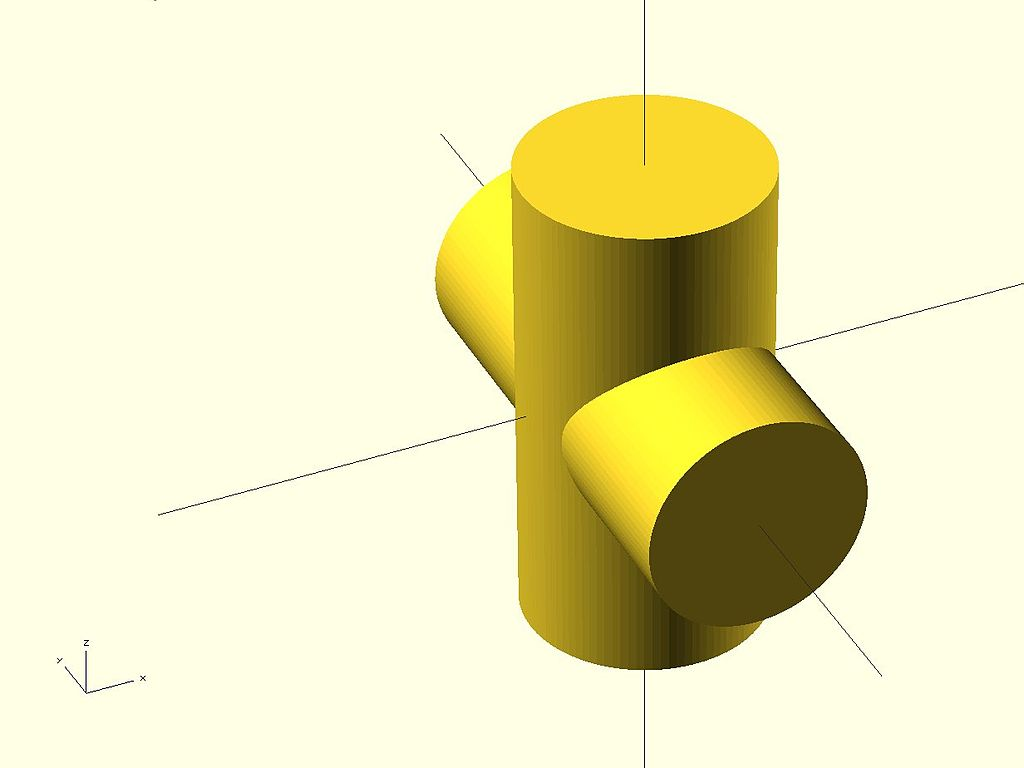
\includegraphics{Imagenes/Openscad_union.jpg}
    \caption{Operación Unión con dos cilindros}
    \label{fig:union_cilindros}
\end{figure}

Código de referencia que muestra la figura \ref{fig:union_cilindros}:\\

\begin{verbatim}
    union() {
 	cylinder (h = 4, r=1, center = true, $fn=100);
 	rotate ([90,0,0]) cylinder (h = 4, r=0.9, center = true, $fn=100);
 }
\end{verbatim}

Es importante mencionar que la unión de los nodos hijos es implícita cuando el comando no es usado. Pero es obligatoria, por ejemplo, en diferencia para agrupar a los primeros nodos hijos en uno.\\

\subsubsection{Diferenccia}

Objetivo: Uso de la operación de Diferencia.\citep{OpenSCS}\\

\subsubsection{Intersección}

Objetivo: Uso de la operación de Intersección.\citep{OpenSCS}\\

\subsection{Simplificación}

\subsubsection{Modulos}

Explicación de la creación de módulos.\citep{OpenSCS}\\

\subsubsection{Funciones}

Objetivo: Explicación del uso de funciones.\citep{OpenSCS}\\

\subsubsection{Include}

Objetivo:\\

Explicación de la inclusión de librerías.\citep{OpenSCS}\\

\subsubsection{Use}

Objetivo:\\

Explicación de el uso de librerías.\citep{OpenSCS}\\

\subsection{Caracteres de Depuración}


\citep{OpenSCS}

\subsection{Matemáticas}


\citep{OpenSCS}

\subsection{Funciones}


\citep{OpenSCS}

\subsection{Misceláneos}


\citep{OpenSCS}



\bibliographystyle{plain}
\bibliography{references}
\end{document}
